\documentclass[aspectratio=169,12pt,t]{beamer}

% --- Theme: Metropolis (modern, clean) ---
\usetheme[progressbar=frametitle,numbering=fraction,block=fill]{metropolis}

% --- Fira Sans font (install texlive-fonts-extra if missing) ---
\IfFileExists{FiraSans.sty}{\usepackage[sfdefault]{FiraSans}}{}

% --- Light background with warm accent ---
\definecolor{mDarkTeal}{RGB}{35,55,59}
\definecolor{mLightBrown}{RGB}{235,228,216}
\definecolor{mAccent}{RGB}{140,70,20}

\setbeamercolor{normal text}{fg=mDarkTeal,bg=white}
\setbeamercolor{alerted text}{fg=mAccent}
\setbeamercolor{frametitle}{bg=mDarkTeal,fg=white}
\setbeamercolor{progress bar}{fg=mAccent,bg=mLightBrown}
\setbeamercolor{title separator}{fg=mAccent}
\setbeamercolor{progress bar in head/foot}{fg=mAccent,bg=mLightBrown}
\setbeamercolor{progress bar in section page}{fg=mAccent,bg=mLightBrown}

% --- Packages ---
\usepackage[utf8]{inputenc}
\usepackage{amsmath,amssymb,amsthm}
\usepackage{mathrsfs}
\usepackage{tikz}
\usetikzlibrary{arrows.meta,positioning,calc,decorations.pathreplacing,shapes,patterns}
\usepackage{pgfplots}
\pgfplotsset{compat=1.18}

% --- TikZ diagram styles (shared across the series) ---
\tikzset{
  axisln/.style={-{Stealth[length=2.6mm]}, line width=0.8pt, gray!75},
  curveln/.style={line width=1.6pt, line cap=round, line join=round},
  projln/.style={dash pattern=on 2.6pt off 2pt, line width=0.7pt},
  guide/.style={-{Stealth[length=2.6mm,width=2.2mm]}, line width=1.1pt},
}
% point marker with a white halo: \dotpt{color}{(coord)}
\newcommand{\dotpt}[2]{%
  \fill[white] #2 circle (3.6pt);
  \fill[#1] #2 circle (2.4pt);
}
% open point marker: \opendotpt{color}{(coord)}
\newcommand{\opendotpt}[2]{%
  \fill[white] #2 circle (3.6pt);
  \draw[#1, line width=1pt] #2 circle (2.4pt);
}

% --- Semi-transparent white highlight for text on top of background images ---
\usepackage[most]{tcolorbox}

% Inline highlight: \hl{short text}
\newtcbox{\hl}{%
  nobeforeafter, tcbox raise base,
  colback=white, opacityback=0.6,
  colframe=white, opacityframe=0,
  sharp corners, boxsep=2pt, left=3pt, right=3pt, top=2pt, bottom=2pt%
}

% Block highlight: \begin{hlbox} ... \end{hlbox}  (multi-line, paragraphs, itemize)
% Optional argument accepts any tcolorbox key, e.g. [width=0.6\linewidth]
\newtcolorbox{hlbox}[1][]{%
  enhanced, breakable,
  colback=white, opacityback=0.6,
  colframe=white, opacityframe=0,
  boxsep=3pt, left=6pt, right=6pt, top=4pt, bottom=4pt,
  sharp corners,
  {#1}%
}

% --- Custom colors for content types ---
\definecolor{defcolor}{RGB}{25,85,120}
\definecolor{thmcolor}{RGB}{140,35,35}
\definecolor{proofcolor}{RGB}{35,100,50}
\definecolor{excolor}{RGB}{140,75,10}
\definecolor{remcolor}{RGB}{90,90,90}

% --- Beamer blocks for mathematical content types (semi-transparent) ---
\tcbset{hlblockbase/.style={
  enhanced, breakable,
  coltitle=white, fonttitle=\bfseries,
  opacitybacktitle=0.8, opacityback=0.6,
  opacityframe=0,
  sharp corners,
  boxsep=1pt, left=5pt, right=5pt, top=2pt, bottom=2pt,
  toptitle=1pt, bottomtitle=1pt
}}

\newtcolorbox{defblock}[1]{hlblockbase, title={#1},
  colbacktitle=defcolor, colback=defcolor!15, colframe=defcolor}
\newtcolorbox{thmblock}[1]{hlblockbase, title={#1},
  colbacktitle=thmcolor, colback=thmcolor!15, colframe=thmcolor}
\newtcolorbox{proofblock}[1]{hlblockbase, title={#1},
  colbacktitle=proofcolor, colback=proofcolor!15, colframe=proofcolor}
\newtcolorbox{exblock}[1]{hlblockbase, title={#1},
  colbacktitle=excolor, colback=excolor!15, colframe=excolor}
\newtcolorbox{remblock}[1]{hlblockbase, title={#1},
  colbacktitle=remcolor, colback=remcolor!15, colframe=remcolor}

% --- Metadata ---
\title{Chapter 5: Differentiation}
\subtitle{Section: The Continuity of Derivatives}
\author{Based on Walter Rudin's \emph{Principles of Mathematical Analysis}}
\date{}

\begin{document}

{
\usebackgroundtemplate{%
  
\includegraphics[width=\paperwidth,height=\paperheight,keepaspectratio=false]{chapter_05_bg_00.png}%
}
\begin{frame}[plain]
  \titlepage

  \note{
    Welcome to Chapter 5, Section 3: The Continuity of Derivatives. In the
    previous section we proved the mean value theorems and learned how the
    derivative controls the global behavior of a function. In this short but
    beautiful episode we ask a different kind of question: how wild can a
    derivative itself be? We already know a derivative need not be
    continuous. But we will prove a remarkable theorem, due to Darboux,
    saying that every derivative still takes all intermediate values, just
    like a continuous function. This puts a real restriction on which
    functions can ever appear as derivatives. Let's dive in.
  }
\end{frame}
}

{
\usebackgroundtemplate{%
  
\includegraphics[width=\paperwidth,height=\paperheight,keepaspectratio=false]{chapter_05_bg_01.png}%
}
\begin{frame}[c]{Outline}
  \begin{center}
    \tableofcontents
  \end{center}

  \note{
    Here is the plan for this episode. We first revisit the surprising
    example from Section 1 of a derivative that exists everywhere but fails
    to be continuous. That raises the question of which functions can be
    derivatives at all. We then state the intermediate value property for
    derivatives, Theorem 5.12, and compare it with the intermediate value
    theorem for continuous functions. After that we walk through the proof
    step by step. Finally we harvest a corollary: a derivative can never
    have a simple discontinuity, only a discontinuity of the second kind.
    We close with a summary and a preview of Lopital's rule.
  }
\end{frame}

\section{Motivation}

% --- Build 1/3 ---
\begin{frame}{How Wild Can a Derivative Be?}
  \begin{hlbox}
  \begin{itemize}
    \item A function $f$ can be differentiable at \alert{every} point,
      yet $f'$ can be \alert{discontinuous} (Example 5.6($b$))
  \end{itemize}
  \end{hlbox}

  \note{
    Let's set the stage. Back in Section 1, Example 5.6, part "b", we met a
    function that is differentiable at every single point of the real line,
    and yet its derivative fails to be continuous at zero. So
    differentiability everywhere does not force the derivative to be a
    continuous function. Next, this raises a natural question.
  }
\end{frame}

% --- Build 2/3 ---
\begin{frame}{How Wild Can a Derivative Be?}
  \begin{hlbox}
  \begin{itemize}
    \item A function $f$ can be differentiable at \alert{every} point,
      yet $f'$ can be \alert{discontinuous} (Example 5.6($b$))
    \item Natural question: is \emph{every} function a derivative?
      \alert{No!}
  \end{itemize}
  \end{hlbox}

  \note{
    So derivatives can be discontinuous. Does that mean anything goes? Could
    any function whatsoever arise as the derivative of some differentiable
    function? The answer is no. Not every function is a derivative.
    Derivatives form a special class of functions, and this section
    identifies one property that every member of that class must have.
  }
\end{frame}

% --- Build 3/3 ---
\begin{frame}{How Wild Can a Derivative Be?}
  \begin{hlbox}
  \begin{itemize}
    \item A function $f$ can be differentiable at \alert{every} point,
      yet $f'$ can be \alert{discontinuous} (Example 5.6($b$))
    \item Natural question: is \emph{every} function a derivative?
      \alert{No!}
    \item Key fact: derivatives on an interval assume
      \alert{intermediate values}, just like continuous functions
      (compare Theorem 4.23)
  \end{itemize}
  \end{hlbox}

  \note{
    Here is the key fact of this section. If "f" prime exists at every point
    of an interval, then "f" prime assumes intermediate values. In other
    words, derivatives share one important property with continuous
    functions, even when they are not continuous themselves. Compare this
    with Theorem 4.23, the intermediate value theorem from Chapter 4. Before
    we state the precise result, let's take another look at the example that
    started this discussion.
  }
\end{frame}

\begin{frame}[c]{Recall Example 5.6($b$): A Discontinuous Derivative}
  \begin{exblock}{Example 5.6($b$)}
    $f(x) = x^2 \sin(1/x)$ for $x \neq 0$, $f(0) = 0$: differentiable
    everywhere, but $f'(x) = 2x\sin(1/x) - \cos(1/x)$ has \alert{no limit}
    as $x \to 0$.
  \end{exblock}

  \begin{center}
  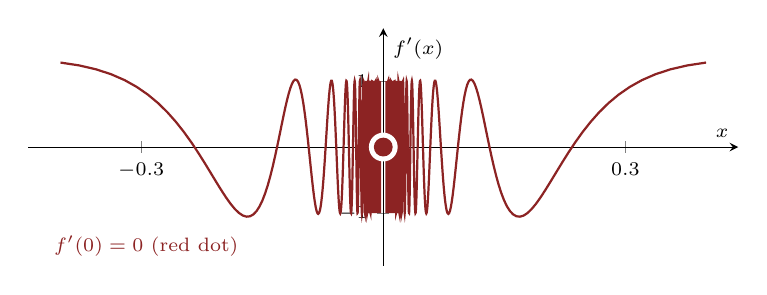
\begin{tikzpicture}
    \begin{axis}[
      width=10.6cm, height=4.6cm,
      axis lines=middle,
      xlabel={$x$}, ylabel={$f'(x)$},
      xmin=-0.44, xmax=0.44, ymin=-1.8, ymax=1.8,
      xtick={-0.3,0.3}, ytick={-1,1},
      tick label style={font=\scriptsize},
      label style={font=\scriptsize},
    ]
      % Parametric substitution u = 1/x: uniform sampling per oscillation,
      % so the curve stays resolved all the way down to |x| = 1/250 = 0.004.
      \addplot[thmcolor, line width=0.8pt, domain=2.5:250, samples=1600,
               variable=\u] ({1/\u}, {(2/\u)*sin(deg(\u)) - cos(deg(\u))});
      \addplot[thmcolor, line width=0.8pt, domain=2.5:250, samples=1600,
               variable=\u] ({-1/\u}, {(2/\u)*sin(deg(\u)) - cos(deg(\u))});
      \fill[white] (axis cs:0,0) circle (5.2pt);
      \fill[thmcolor] (axis cs:0,0) circle (3.4pt);
      \node[thmcolor, font=\scriptsize, anchor=west]
        at (axis cs:-0.42,-1.5) {$f'(0)=0$ (red dot)};
    \end{axis}
  \end{tikzpicture}
  \end{center}

  \note{
    As you can see on the slide, the function "f" of "x" equals "x" squared
    times sine of one over "x", with "f" of zero equal to zero, is
    differentiable at every point, and "f" prime of zero equals zero. The
    picture shows the graph of the derivative in red. Away from zero it is a
    nice smooth curve, but as "x" approaches zero the cosine term makes the
    derivative oscillate between values near minus one and plus one, faster
    and faster, without ever settling down. The oscillation becomes so rapid
    that near the origin the graph merges into a solid band of red; the
    individual waves are simply too thin to draw. The red dot at the origin marks
    the value "f" prime of zero, which equals zero. So the derivative is
    defined everywhere, but it has no limit at zero, and it is
    discontinuous there. Notice, though, that the
    derivative does not jump over any values; it keeps sweeping through
    them. That observation is exactly what the next theorem captures.
  }
\end{frame}

}

{
\usebackgroundtemplate{%
  
\includegraphics[width=\paperwidth,height=\paperheight,keepaspectratio=false]{chapter_05_bg_02.png}%
}
\section{The Intermediate Value Property}

\begin{frame}[c]{Recall: The Intermediate Value Theorem}
  \begin{remblock}{Recall: Theorem 4.23}
    If $f$ is \emph{continuous} on $[a, b]$ and $f(a) < c < f(b)$, then
    $f(x) = c$ for some $x \in (a, b)$.
  \end{remblock}

  \begin{center}
  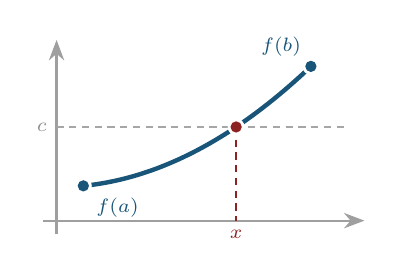
\begin{tikzpicture}[scale=0.85]
    \draw[axisln] (-0.2,0) -- (4.6,0);
    \draw[axisln] (0,-0.2) -- (0,2.7);
    \draw[curveln, defcolor, domain=0.4:3.8, smooth, samples=60]
      plot (\x, {0.5 + 0.125*\x*\x});
    \draw[gray!70, projln] (0,1.4) -- (4.3,1.4);
    \node[gray!90, left, font=\scriptsize] at (0,1.4) {$c$};
    \dotpt{defcolor}{(0.4,0.52)}
    \dotpt{defcolor}{(3.8,2.305)}
    \node[defcolor, below right, font=\scriptsize] at (0.45,0.48) {$f(a)$};
    \node[defcolor, above left, font=\scriptsize] at (3.8,2.31) {$f(b)$};
    \draw[thmcolor, projln] (2.683,1.4) -- (2.683,0);
    \dotpt{thmcolor}{(2.683,1.4)}
    \node[thmcolor, below, font=\scriptsize] at (2.683,0) {$x$};
  \end{tikzpicture}
  \end{center}

  \note{
    First, a quick reminder of the intermediate value theorem for continuous
    functions, Theorem 4.23 from Chapter 4. If "f" is continuous on the
    closed interval from "a" to "b", and "c" is any value strictly between
    "f" of "a" and "f" of "b", then "f" actually attains the value "c"
    somewhere inside the interval. In the picture, the blue curve is the
    graph of a continuous function, the dashed horizontal line is the level
    "c", and the red point marks the place "x" where the graph crosses that
    level. The proof used connectedness: a continuous image of an interval
    is an interval, so no values can be skipped. Now for the surprise: the
    same conclusion holds for derivatives, even discontinuous ones.
  }
\end{frame}

\begin{frame}{Theorem 5.12: Derivatives Assume Intermediate Values}
  \begin{thmblock}{Theorem 5.12 (Darboux)}
    Suppose $f$ is a real differentiable function on $[a, b]$ and
    $f'(a) < \lambda < f'(b)$. Then there is a point $x \in (a, b)$
    such that $f'(x) = \lambda$.
  \end{thmblock}

  \vspace{0.5em}
  \begin{hlbox}
  \begin{itemize}
    \item A similar result holds if $f'(a) > f'(b)$
    \item \textbf{Note:} we assume \alert{nothing} about the continuity
      of $f'$!
  \end{itemize}
  \end{hlbox}

  \note{
    Here is the main theorem of this section, often called Darboux's
    theorem. Suppose "f" is differentiable at every point of the closed
    interval from "a" to "b", and suppose lambda is any number strictly
    between "f" prime of "a" and "f" prime of "b". Then the derivative
    actually takes the value lambda at some interior point "x". The first
    bullet notes that the symmetric case works the same way: if "f" prime
    of "a" is larger than "f" prime of "b", the same conclusion holds. The
    second bullet is the remarkable part. We assume only that the
    derivative exists everywhere. We do not assume it is continuous, so we
    cannot simply apply the intermediate value theorem to "f" prime. Let's
    draw a picture of what the theorem says.
  }
\end{frame}

\begin{frame}[c]{Theorem 5.12: The Picture}
  \begin{center}
  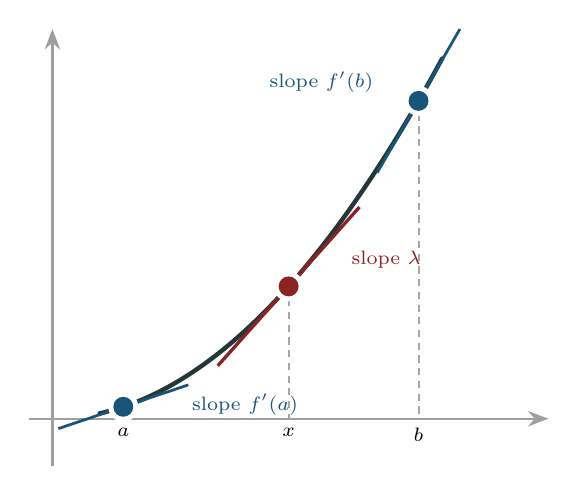
\begin{tikzpicture}[scale=1.5]
    \draw[axisln] (-0.2,0) -- (4.2,0);
    \draw[axisln] (0,-0.4) -- (0,3.3);
    \draw[curveln, mDarkTeal, domain=0.4:3.3, smooth, samples=60]
      plot (\x, {0.28*\x*\x});
    % tangent at a (slope 0.336)
    \draw[defcolor, line width=1pt] (0.05,-0.084) -- (1.15,0.286);
    % tangent at b (slope 1.736)
    \draw[defcolor, line width=1pt] (2.75,2.083) -- (3.45,3.299);
    % tangent at x (slope 1.12)
    \draw[thmcolor, line width=1.2pt] (1.4,0.448) -- (2.6,1.792);
    % projections
    \draw[gray!70, projln] (0.6,0.101) -- (0.6,0);
    \draw[gray!70, projln] (2.0,1.12) -- (2.0,0);
    \draw[gray!70, projln] (3.1,2.691) -- (3.1,0);
    \dotpt{defcolor}{(0.6,0.101)}
    \dotpt{defcolor}{(3.1,2.691)}
    \dotpt{thmcolor}{(2.0,1.12)}
    \node[below, font=\scriptsize] at (0.6,0) {$a$};
    \node[below, font=\scriptsize] at (2.0,0) {$x$};
    \node[below, font=\scriptsize] at (3.1,0) {$b$};
    \node[defcolor, right, font=\scriptsize] at (1.1,0.12) {slope $f'(a)$};
    \node[defcolor, left, font=\scriptsize] at (2.8,2.85) {slope $f'(b)$};
    \node[thmcolor, right, font=\scriptsize] at (2.45,1.35)
      {slope $\lambda$};
  \end{tikzpicture}
  \end{center}

  \note{
    Let's look at the picture. The dark curve is the graph of "f". At the
    left endpoint "a", the blue tangent line is fairly flat: the slope
    there is "f" prime of "a", which is small. At the right endpoint "b",
    the blue tangent is much steeper: the slope is "f" prime of "b". Now
    pick any target slope lambda strictly in between. The theorem promises
    a point "x" between "a" and "b", marked in red, where the tangent line
    has exactly the slope lambda. Intuitively, as we slide along the curve
    from "a" to "b", the tangent slope cannot skip over any intermediate
    value, even if it varies in a discontinuous way. Let's now see how to
    prove this.
  }
\end{frame}

}

{
\usebackgroundtemplate{%
  
\includegraphics[width=\paperwidth,height=\paperheight,keepaspectratio=false]{chapter_05_bg_03.png}%
}
\section{Proof of Theorem 5.12}

\begin{frame}{Proof Strategy: Theorem 5.12}
  \begin{hlbox}
  \textbf{Goal:} Find $x \in (a, b)$ with $f'(x) = \lambda$.

  \vspace{0.8em}
  \textbf{Approach:}
  \begin{enumerate}
    \item Tilt the picture:\\
      study $g(t) = f(t) - \lambda t$, so the target
      slope becomes $g'(x) = 0$
    \item Show neither endpoint can be a minimum of $g$
      (using $g'(a) < 0 < g'(b)$)
    \item $g$ is continuous on the compact set $[a, b]$, so it attains a
      minimum (Theorem 4.16) --- necessarily at an \alert{interior} point
    \item At an interior minimum, $g'(x) = 0$ (Theorem 5.8)
  \end{enumerate}
  \end{hlbox}

  \note{
    Before writing the formal proof, let's understand the strategy. Step 1
    is a standard trick: subtract lambda times "t" from "f" of "t" to get
    an auxiliary function "g". This tilts the picture so that finding a
    point where "f" prime equals lambda becomes finding a point where "g"
    prime equals zero. Step 2 shows that "g" dips below its value at each
    endpoint, so no endpoint can be where "g" is smallest. Step 3 invokes
    compactness: a continuous function on a closed bounded interval attains
    its minimum somewhere, and by step 2 that somewhere must be an interior
    point. Step 4 is the result from Section 2 that at an interior minimum
    the derivative vanishes. Chaining these together finishes the proof.
    Let's first see this plan in a picture.
  }
\end{frame}

\begin{frame}[c]{Proof: The Picture}
  \begin{center}
  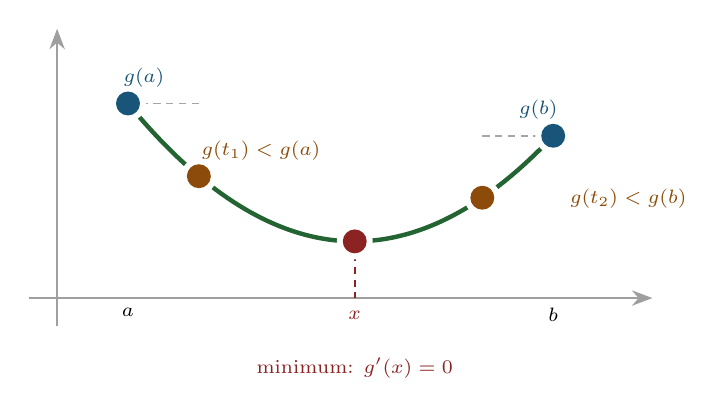
\begin{tikzpicture}[scale=1.8]
    \draw[axisln] (-0.2,0) -- (4.2,0);
    \draw[axisln] (0,-0.2) -- (0,1.9);
    \draw[curveln, proofcolor, domain=0.5:3.5, smooth, samples=60]
      plot (\x, {0.4 + 0.38*(\x-2.1)*(\x-2.1)});
    % endpoint levels
    \draw[gray!70, projln] (0.5,1.373) -- (1.0,1.373);
    \draw[gray!70, projln] (3.5,1.145) -- (3.0,1.145);
    \dotpt{defcolor}{(0.5,1.373)}
    \dotpt{defcolor}{(3.5,1.145)}
    \node[defcolor, above right, font=\scriptsize] at (0.4,1.42) {$g(a)$};
    \node[defcolor, above left, font=\scriptsize] at (3.6,1.19) {$g(b)$};
    % dips below the endpoints
    \dotpt{excolor}{(1.0,0.86)}
    \dotpt{excolor}{(3.0,0.708)}
    \node[excolor, above right, font=\scriptsize] at (0.95,0.9)
      {$g(t_1) < g(a)$};
    \node[excolor, right, font=\scriptsize] at (3.55,0.7)
      {$g(t_2) < g(b)$};
    % interior minimum
    \draw[thmcolor, projln] (2.1,0.4) -- (2.1,0);
    \dotpt{thmcolor}{(2.1,0.4)}
    \node[thmcolor, below, font=\scriptsize] at (2.1,-0.02) {$x$};
    \node[thmcolor, below, font=\scriptsize] at (2.1,-0.35)
      {minimum: $g'(x)=0$};
    \node[below, font=\scriptsize] at (0.5,0) {$a$};
    \node[below, font=\scriptsize] at (3.5,0) {$b$};
  \end{tikzpicture}
  \end{center}

  \note{
    Here is the whole proof in one picture. The green curve is the graph of
    the auxiliary function "g" on the interval from "a" to "b". Because "g"
    prime of "a" is negative, the curve starts by heading downward, so just
    to the right of "a" there is a point "t" sub 1, marked in orange, where
    "g" is strictly below "g" of "a". Symmetrically, because "g" prime of
    "b" is positive, the curve rises into "b", so there is a point "t" sub
    2 where "g" is strictly below "g" of "b". So the smallest value of "g"
    is not at either endpoint. The minimum, marked in red at the point "x",
    must lie strictly inside the interval, and there the derivative of "g"
    is zero. Now let's carry out each step carefully.
  }
\end{frame}

% --- Build 1/5 ---
\begin{frame}{Proof of Theorem 5.12}
  \begin{proofblock}{Step 1: The tilted function}
    Put $g(t) = f(t) - \lambda t$. Then $g$ is differentiable on
    $[a, b]$ and
    \[
      g'(t) = f'(t) - \lambda, \qquad
      g'(a) < 0, \quad g'(b) > 0.
    \]
  \end{proofblock}

  \note{
    Step 1. We define the tilted function "g" of "t" equals "f" of "t"
    minus lambda times "t". Differentiating, "g" prime equals "f" prime
    minus lambda. Since lambda lies strictly between "f" prime of "a" and
    "f" prime of "b", we get "g" prime of "a" negative and "g" prime of "b"
    positive. Our goal is now to find an interior point where "g" prime
    vanishes, because that is exactly where "f" prime equals lambda.
  }
\end{frame}

% --- Build 2/5 ---
\begin{frame}{Proof of Theorem 5.12}
  \begin{proofblock}{Step 2: $a$ is not a minimum of $g$}
    $g'(a) < 0$ means
    $\displaystyle \lim_{t \to a} \frac{g(t) - g(a)}{t - a} < 0$,
    so for some $t_1 \in (a, b)$:
    \[
      \boxed{g(t_1) < g(a)}
    \]
  \end{proofblock}

  \note{
    Step 2. We claim the left endpoint is not a minimum of "g". Look at the
    difference quotient on the slide: it converges to "g" prime of "a",
    which is negative. So for "t" close enough to "a" the quotient itself
    is negative. But the denominator, "t" minus "a", is positive, so the
    numerator must be negative. That gives a point "t" sub 1 where "g" is
    strictly smaller than "g" of "a". Note the subtle point: we only know
    the derivative at the single point "a", so we cannot say "g" is
    decreasing on an interval; but one point below "g" of "a" is all we
    need. Next, the right endpoint.
  }
\end{frame}

% --- Build 3/5 ---
\begin{frame}{Proof of Theorem 5.12}
  \begin{proofblock}{Step 3: $b$ is not a minimum of $g$}
    Similarly, $g'(b) > 0$ means
    $\displaystyle \lim_{t \to b} \frac{g(t) - g(b)}{t - b} > 0$,
    and now $t - b < 0$, so for some $t_2 \in (a, b)$:
    \[
      \boxed{g(t_2) < g(b)}
    \]
  \end{proofblock}

  \note{
    Step 3 is the mirror image. The difference quotient at "b" converges to
    "g" prime of "b", which is positive, so it is positive for "t" close to
    "b". This time the denominator, "t" minus "b", is negative, so the
    numerator must be negative as well. That produces a point "t" sub 2
    where "g" is strictly below "g" of "b". So neither endpoint achieves
    the smallest value of "g". Now compactness enters.
  }
\end{frame}

% --- Build 4/5 ---
\begin{frame}{Proof of Theorem 5.12}
  \begin{proofblock}{Step 4: $g$ attains an interior minimum}
    $g$ is continuous on the compact set $[a, b]$, so it attains its
    minimum at some point $x \in [a, b]$ (Theorem 4.16).
    By Steps 2 and 3, $x \neq a$ and $x \neq b$:
    \[
      \boxed{a < x < b}
    \]
  \end{proofblock}

  \note{
    Step 4. The function "g" is differentiable, hence continuous, and the
    closed interval from "a" to "b" is compact. Recall Theorem 4.16: a
    continuous real function on a compact set attains its minimum. So there
    is a point "x" in the interval where "g" is smallest. Could that point
    be an endpoint? No. Step 2 gave us a value of "g" strictly below "g" of
    "a", and step 3 gave one strictly below "g" of "b". So the minimum
    point "x" lies strictly between "a" and "b". One step remains.
  }
\end{frame}

% --- Build 5/5 ---
\begin{frame}{Proof of Theorem 5.12}
  \begin{proofblock}{Step 5: Conclusion}
    $g$ has a local minimum at the interior point $x$ and $g'(x)$ exists,
    so $g'(x) = 0$ (Theorem 5.8). Hence
    \[
      \boxed{f'(x) = \lambda} \qquad \blacksquare
    \]
  \end{proofblock}

  \note{
    Step 5, the conclusion. The point "x" is an interior minimum of "g",
    and "g" is differentiable there. By Theorem 5.8 from the previous
    section, the derivative at an interior extremum must vanish, so "g"
    prime of "x" equals zero. Since "g" prime equals "f" prime minus
    lambda, this says exactly that "f" prime of "x" equals lambda, and the
    proof is complete. Notice how the proof never needed continuity of the
    derivative; it only used the existence of the derivative at every
    point, plus compactness. Let's now collect the consequences.
  }
\end{frame}

}

{
\usebackgroundtemplate{%
  
\includegraphics[width=\paperwidth,height=\paperheight,keepaspectratio=false]{chapter_05_bg_04.png}%
}
\section{Consequences}

\begin{frame}{Recall: Two Kinds of Discontinuity}
  \begin{remblock}{Recall: Definition 4.26}
    Let $f$ have a discontinuity at $x$.
    \begin{itemize}
      \item \textbf{Simple discontinuity (first kind):} $f(x+)$ and
        $f(x-)$ both exist
      \item \textbf{Discontinuity of the second kind:} $f(x+)$ or
        $f(x-)$ fails to exist
    \end{itemize}
  \end{remblock}

  \note{
    To appreciate the corollary, recall Definition 4.26 from Chapter 4,
    which classifies discontinuities into two kinds. A simple
    discontinuity, also called a discontinuity of the first kind, is one
    where both one sided limits exist; the function jumps from one value to
    another, or has both limits equal but different from the function
    value. A discontinuity of the second kind is one where at least one of
    the one sided limits fails to exist entirely, for example because the
    function oscillates. With this language in place, here is what Theorem
    5.12 tells us about derivatives.
  }
\end{frame}

\begin{frame}{Corollary: No Simple Discontinuities}
  \begin{thmblock}{Corollary (to Theorem 5.12)}
    If $f$ is differentiable on $[a, b]$, then $f'$ cannot have any
    \alert{simple} discontinuities on $[a, b]$.
  \end{thmblock}

  \vspace{0.5em}
  \begin{hlbox}
  \textbf{Key idea:} a jump in $f'$ would force $f'$ to \alert{skip}
  intermediate values --- impossible by Theorem 5.12.
  \end{hlbox}

  \note{
    Here is the corollary. If "f" is differentiable on the whole interval,
    then its derivative cannot have any simple discontinuities. In other
    words, a derivative can never jump. The key idea is on the slide: at a
    jump, the one sided limits of "f" prime exist but leave a gap, and
    every value inside that gap would be skipped by "f" prime near the
    jump point. But Theorem 5.12 says a derivative can never skip
    intermediate values. Let's make this picture explicit on the next
    slide.
  }
\end{frame}

\begin{frame}[c]{Why a Jump in $f'$ Is Impossible}
  \begin{center}
  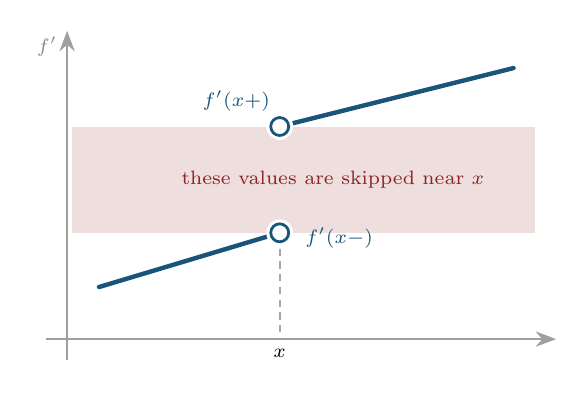
\begin{tikzpicture}[scale=1.35]
    % skipped band (behind everything)
    \fill[thmcolor!15] (0.05,1.0) rectangle (4.4,2.0);
    \draw[axisln] (-0.2,0) -- (4.6,0);
    \draw[axisln] (0,-0.2) -- (0,2.9);
    \node[gray!90, left, font=\scriptsize] at (0,2.75) {$f'$};
    % left branch
    \draw[curveln, defcolor, domain=0.3:2.0] plot (\x, {0.4 + 0.3*\x});
    % right branch
    \draw[curveln, defcolor, domain=2.0:4.2] plot (\x, {2.0 + 0.25*(\x-2)});
    \draw[gray!70, projln] (2.0,0.85) -- (2.0,0);
    \opendotpt{defcolor}{(2.0,1.0)}
    \opendotpt{defcolor}{(2.0,2.0)}
    \node[below, font=\scriptsize] at (2.0,0) {$x$};
    \node[defcolor, right, font=\scriptsize] at (2.15,0.95) {$f'(x-)$};
    \node[defcolor, above left, font=\scriptsize] at (2.0,2.05) {$f'(x+)$};
    \node[thmcolor, font=\scriptsize] at (2.5,1.5)
      {these values are \alert{skipped} near $x$};
  \end{tikzpicture}
  \end{center}

  \vspace{-0.3em}
  \begin{hlbox}
  Values between $f'(x-)$ and $f'(x+)$ are never attained near $x$
  --- contradicting Theorem 5.12.
  \end{hlbox}

  \note{
    Here is the picture of an impossible situation. The blue curve shows a
    hypothetical derivative with a jump at the point "x": approaching from
    the left, the values tend to the lower open circle, the left hand limit;
    approaching from the right, they tend to the upper open circle, the
    right hand limit. The dashed line drops from the lower circle down to
    the point "x" on the horizontal axis, marking where the jump happens.
    The shaded pink band between the two circles is the gap. Near "x",
    the hypothetical derivative takes values just below the band on the
    left side and just above the band on the right side, but nothing inside
    the band. Now apply Theorem 5.12 on a small interval around "x": any
    value in the band lies between two attained derivative values, so it
    would have to be attained. Contradiction. So a derivative simply cannot
    jump.
  }
\end{frame}

\begin{frame}{But the Second Kind Can Happen}
  \begin{remblock}{Remark}
    $f'$ \emph{may} very well have discontinuities of the
    \alert{second kind}.
  \end{remblock}

  \vspace{0.5em}
  \begin{hlbox}
  \begin{itemize}
    \item Example 5.6($b$): $f'(x) = 2x\sin(1/x) - \cos(1/x)$
      \alert{oscillates} as $x \to 0$
    \item Neither $f'(0+)$ nor $f'(0-)$ exists --- yet no intermediate
      value is skipped
  \end{itemize}
  \end{hlbox}

  \note{
    A word of caution: the corollary rules out only simple
    discontinuities. Discontinuities of the second kind can and do occur.
    Our running example, Example 5.6, part "b", is exactly of this type.
    The first bullet recalls its derivative, which oscillates without
    settling down as "x" approaches zero. The second bullet points out that
    neither one sided limit exists at zero, so this is a discontinuity of
    the second kind, and there is no conflict with Theorem 5.12, because
    the wild oscillation sweeps through all the intermediate values instead
    of skipping any. So the picture is consistent: derivatives may
    oscillate badly, but they may never jump. Let's summarize.
  }
\end{frame}

}

{
\usebackgroundtemplate{%
  
\includegraphics[width=\paperwidth,height=\paperheight,keepaspectratio=false]{chapter_05_bg_05.png}%
}
\section{Summary}

% --- Build 1/3 ---
\begin{frame}{Summary}
  \begin{hlbox}
  \textbf{Key takeaways from this section:}
  \begin{itemize}
    \item \textbf{Theorem 5.12 (Darboux):} if $f$ is differentiable on
      $[a, b]$, then $f'$ assumes every value between $f'(a)$ and $f'(b)$
  \end{itemize}
  \end{hlbox}

  \note{
    Let's review what we covered. The centerpiece was Theorem 5.12, often
    called Darboux's theorem: if "f" is differentiable on a closed
    interval, then its derivative assumes every value between "f" prime of
    "a" and "f" prime of "b", with no continuity assumption on the
    derivative whatsoever. The proof tilted the function, used compactness
    to find an interior minimum, and applied the vanishing derivative
    theorem from Section 2.
  }
\end{frame}

% --- Build 2/3 ---
\begin{frame}{Summary}
  \begin{hlbox}
  \textbf{Key takeaways from this section:}
  \begin{itemize}
    \item \textbf{Theorem 5.12 (Darboux):} if $f$ is differentiable on
      $[a, b]$, then $f'$ assumes every value between $f'(a)$ and $f'(b)$
    \item \textbf{Corollary:} $f'$ has \alert{no simple discontinuities}
      --- a derivative can never jump
  \end{itemize}
  \end{hlbox}

  \note{
    As a corollary, a derivative can never have a simple discontinuity. A
    jump in the derivative would leave a gap of skipped values, and
    Darboux's theorem forbids skipping. This is a genuine restriction on
    which functions can be derivatives: for example, a step function is
    continuous except for one innocent jump, yet it is not the derivative
    of anything on an interval containing that jump.
  }
\end{frame}

% --- Build 3/3 ---
\begin{frame}{Summary}
  \begin{hlbox}
  \textbf{Key takeaways from this section:}
  \begin{itemize}
    \item \textbf{Theorem 5.12 (Darboux):} if $f$ is differentiable on
      $[a, b]$, then $f'$ assumes every value between $f'(a)$ and $f'(b)$
    \item \textbf{Corollary:} $f'$ has \alert{no simple discontinuities}
      --- a derivative can never jump
    \item But $f'$ \emph{can} have discontinuities of the
      \alert{second kind} (oscillation, as in Example 5.6($b$))
  \end{itemize}

  \vspace{0.8em}
  \textbf{Coming up next:} L'Hospital's Rule --- computing limits of
  quotients via derivatives.
  \end{hlbox}

  \note{
    On the other hand, discontinuities of the second kind are possible:
    Example 5.6, part "b", gave a derivative that oscillates so wildly near
    zero that no one sided limit exists. So derivatives occupy a curious
    middle ground: not necessarily continuous, but never jumping. In the
    next episode we put the generalized mean value theorem to work and
    prove one of the most practical results of the chapter, Lopital's
    rule, which lets us compute limits of quotients by differentiating the
    numerator and the denominator. See you there.
  }
\end{frame}
}

\end{document}
